% The three-step factorization of (p) as it climbs ℚ → K^D → K^I → K:
% first splitting into g primes, then inert (degree grows to f), then
% ramifying with exponent e.
% Source: book/tex/alg-NT/ramification.tex (§ (Optional)
% Decomposition and inertia groups) — tikzcd.
\documentclass[border=2mm]{standalone}
\usepackage{tikz}
\usetikzlibrary{arrows.meta}
\usepackage{amssymb}
\begin{document}
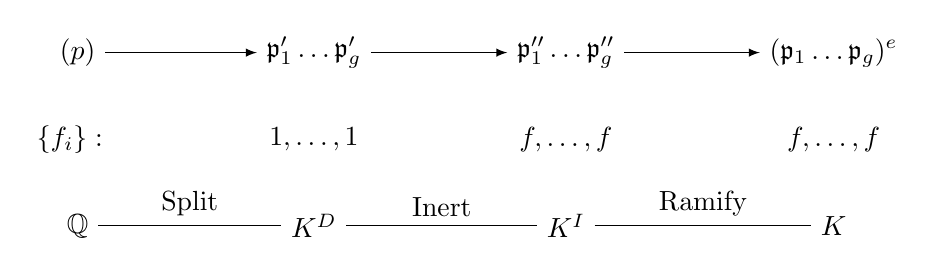
\begin{tikzpicture}[>=latex]
  \node (p) at (0,2.2) {$(p)$};
  \node (a) at (3.0,2.2) {$\mathfrak{p}'_1 \dots \mathfrak{p}'_g$};
  \node (b) at (6.2,2.2) {$\mathfrak{p}''_1 \dots \mathfrak{p}''_g$};
  \node (c) at (9.6,2.2) {$(\mathfrak{p}_1 \dots \mathfrak{p}_g)^e$};
  \draw[->] (p) -- (a);
  \draw[->] (a) -- (b);
  \draw[->] (b) -- (c);
  \node at (-0.1,1.1) {$\{f_i\}:$};
  \node at (3.0,1.1) {$1,\dots,1$};
  \node at (6.2,1.1) {$f,\dots,f$};
  \node at (9.6,1.1) {$f,\dots,f$};
  \node (Q) at (0,0) {$\mathbb{Q}$};
  \node (KD) at (3.0,0) {$K^D$};
  \node (KI) at (6.2,0) {$K^I$};
  \node (K) at (9.6,0) {$K$};
  \draw (Q) -- (KD) node[midway,above] {Split};
  \draw (KD) -- (KI) node[midway,above] {Inert};
  \draw (KI) -- (K) node[midway,above] {Ramify};
\end{tikzpicture}
\end{document}
